% Graphic for TeX using PGF
% Title: /home/satenske/cours/AP/obj3/TD1/1.dia
% Creator: Dia v0.97.1
% CreationDate: Thu Oct 20 08:31:56 2011
% For: satenske
% \usepackage{tikz}
% The following commands are not supported in PSTricks at present
% We define them conditionally, so when they are implemented,
% this pgf file will use them.
\ifx\du\undefined
  \newlength{\du}
\fi
\setlength{\du}{15\unitlength}
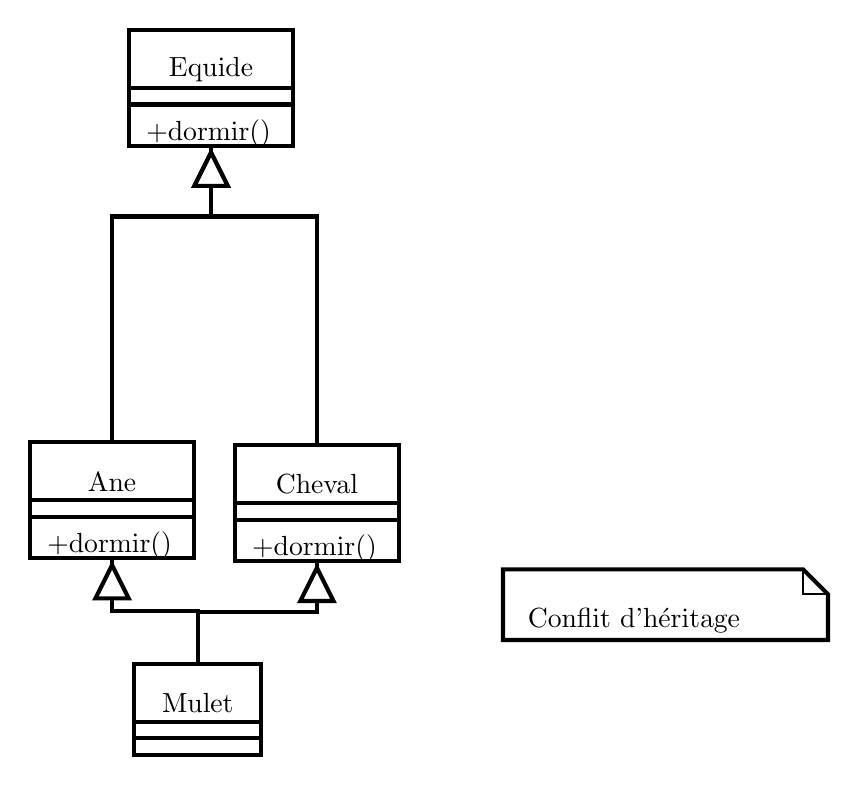
\begin{tikzpicture}
\pgftransformxscale{1.000000}
\pgftransformyscale{-1.000000}
\definecolor{dialinecolor}{rgb}{0.000000, 0.000000, 0.000000}
\pgfsetstrokecolor{dialinecolor}
\definecolor{dialinecolor}{rgb}{1.000000, 1.000000, 1.000000}
\pgfsetfillcolor{dialinecolor}
\pgfsetlinewidth{0.100000\du}
\pgfsetdash{}{0pt}
\definecolor{dialinecolor}{rgb}{1.000000, 1.000000, 1.000000}
\pgfsetfillcolor{dialinecolor}
\fill (18.150000\du,2.250000\du)--(18.150000\du,3.650000\du)--(22.115000\du,3.650000\du)--(22.115000\du,2.250000\du)--cycle;
\definecolor{dialinecolor}{rgb}{0.000000, 0.000000, 0.000000}
\pgfsetstrokecolor{dialinecolor}
\draw (18.150000\du,2.250000\du)--(18.150000\du,3.650000\du)--(22.115000\du,3.650000\du)--(22.115000\du,2.250000\du)--cycle;
% setfont left to latex
\definecolor{dialinecolor}{rgb}{0.000000, 0.000000, 0.000000}
\pgfsetstrokecolor{dialinecolor}
\node at (20.132500\du,3.200000\du){Equide};
\definecolor{dialinecolor}{rgb}{1.000000, 1.000000, 1.000000}
\pgfsetfillcolor{dialinecolor}
\fill (18.150000\du,3.650000\du)--(18.150000\du,4.050000\du)--(22.115000\du,4.050000\du)--(22.115000\du,3.650000\du)--cycle;
\definecolor{dialinecolor}{rgb}{0.000000, 0.000000, 0.000000}
\pgfsetstrokecolor{dialinecolor}
\draw (18.150000\du,3.650000\du)--(18.150000\du,4.050000\du)--(22.115000\du,4.050000\du)--(22.115000\du,3.650000\du)--cycle;
\definecolor{dialinecolor}{rgb}{1.000000, 1.000000, 1.000000}
\pgfsetfillcolor{dialinecolor}
\fill (18.150000\du,4.050000\du)--(18.150000\du,5.050000\du)--(22.115000\du,5.050000\du)--(22.115000\du,4.050000\du)--cycle;
\definecolor{dialinecolor}{rgb}{0.000000, 0.000000, 0.000000}
\pgfsetstrokecolor{dialinecolor}
\draw (18.150000\du,4.050000\du)--(18.150000\du,5.050000\du)--(22.115000\du,5.050000\du)--(22.115000\du,4.050000\du)--cycle;
% setfont left to latex
\definecolor{dialinecolor}{rgb}{0.000000, 0.000000, 0.000000}
\pgfsetstrokecolor{dialinecolor}
\node[anchor=west] at (18.300000\du,4.750000\du){+dormir()};
\pgfsetlinewidth{0.100000\du}
\pgfsetdash{}{0pt}
\definecolor{dialinecolor}{rgb}{1.000000, 1.000000, 1.000000}
\pgfsetfillcolor{dialinecolor}
\fill (20.700000\du,12.250000\du)--(20.700000\du,13.650000\du)--(24.665000\du,13.650000\du)--(24.665000\du,12.250000\du)--cycle;
\definecolor{dialinecolor}{rgb}{0.000000, 0.000000, 0.000000}
\pgfsetstrokecolor{dialinecolor}
\draw (20.700000\du,12.250000\du)--(20.700000\du,13.650000\du)--(24.665000\du,13.650000\du)--(24.665000\du,12.250000\du)--cycle;
% setfont left to latex
\definecolor{dialinecolor}{rgb}{0.000000, 0.000000, 0.000000}
\pgfsetstrokecolor{dialinecolor}
\node at (22.682500\du,13.200000\du){Cheval};
\definecolor{dialinecolor}{rgb}{1.000000, 1.000000, 1.000000}
\pgfsetfillcolor{dialinecolor}
\fill (20.700000\du,13.650000\du)--(20.700000\du,14.050000\du)--(24.665000\du,14.050000\du)--(24.665000\du,13.650000\du)--cycle;
\definecolor{dialinecolor}{rgb}{0.000000, 0.000000, 0.000000}
\pgfsetstrokecolor{dialinecolor}
\draw (20.700000\du,13.650000\du)--(20.700000\du,14.050000\du)--(24.665000\du,14.050000\du)--(24.665000\du,13.650000\du)--cycle;
\definecolor{dialinecolor}{rgb}{1.000000, 1.000000, 1.000000}
\pgfsetfillcolor{dialinecolor}
\fill (20.700000\du,14.050000\du)--(20.700000\du,15.050000\du)--(24.665000\du,15.050000\du)--(24.665000\du,14.050000\du)--cycle;
\definecolor{dialinecolor}{rgb}{0.000000, 0.000000, 0.000000}
\pgfsetstrokecolor{dialinecolor}
\draw (20.700000\du,14.050000\du)--(20.700000\du,15.050000\du)--(24.665000\du,15.050000\du)--(24.665000\du,14.050000\du)--cycle;
% setfont left to latex
\definecolor{dialinecolor}{rgb}{0.000000, 0.000000, 0.000000}
\pgfsetstrokecolor{dialinecolor}
\node[anchor=west] at (20.850000\du,14.750000\du){+dormir()};
\pgfsetlinewidth{0.100000\du}
\pgfsetdash{}{0pt}
\definecolor{dialinecolor}{rgb}{1.000000, 1.000000, 1.000000}
\pgfsetfillcolor{dialinecolor}
\fill (15.765000\du,12.185000\du)--(15.765000\du,13.585000\du)--(19.730000\du,13.585000\du)--(19.730000\du,12.185000\du)--cycle;
\definecolor{dialinecolor}{rgb}{0.000000, 0.000000, 0.000000}
\pgfsetstrokecolor{dialinecolor}
\draw (15.765000\du,12.185000\du)--(15.765000\du,13.585000\du)--(19.730000\du,13.585000\du)--(19.730000\du,12.185000\du)--cycle;
% setfont left to latex
\definecolor{dialinecolor}{rgb}{0.000000, 0.000000, 0.000000}
\pgfsetstrokecolor{dialinecolor}
\node at (17.747500\du,13.135000\du){Ane};
\definecolor{dialinecolor}{rgb}{1.000000, 1.000000, 1.000000}
\pgfsetfillcolor{dialinecolor}
\fill (15.765000\du,13.585000\du)--(15.765000\du,13.985000\du)--(19.730000\du,13.985000\du)--(19.730000\du,13.585000\du)--cycle;
\definecolor{dialinecolor}{rgb}{0.000000, 0.000000, 0.000000}
\pgfsetstrokecolor{dialinecolor}
\draw (15.765000\du,13.585000\du)--(15.765000\du,13.985000\du)--(19.730000\du,13.985000\du)--(19.730000\du,13.585000\du)--cycle;
\definecolor{dialinecolor}{rgb}{1.000000, 1.000000, 1.000000}
\pgfsetfillcolor{dialinecolor}
\fill (15.765000\du,13.985000\du)--(15.765000\du,14.985000\du)--(19.730000\du,14.985000\du)--(19.730000\du,13.985000\du)--cycle;
\definecolor{dialinecolor}{rgb}{0.000000, 0.000000, 0.000000}
\pgfsetstrokecolor{dialinecolor}
\draw (15.765000\du,13.985000\du)--(15.765000\du,14.985000\du)--(19.730000\du,14.985000\du)--(19.730000\du,13.985000\du)--cycle;
% setfont left to latex
\definecolor{dialinecolor}{rgb}{0.000000, 0.000000, 0.000000}
\pgfsetstrokecolor{dialinecolor}
\node[anchor=west] at (15.915000\du,14.685000\du){+dormir()};
\pgfsetlinewidth{0.100000\du}
\pgfsetdash{}{0pt}
\definecolor{dialinecolor}{rgb}{1.000000, 1.000000, 1.000000}
\pgfsetfillcolor{dialinecolor}
\fill (18.280000\du,17.520000\du)--(18.280000\du,18.920000\du)--(21.345000\du,18.920000\du)--(21.345000\du,17.520000\du)--cycle;
\definecolor{dialinecolor}{rgb}{0.000000, 0.000000, 0.000000}
\pgfsetstrokecolor{dialinecolor}
\draw (18.280000\du,17.520000\du)--(18.280000\du,18.920000\du)--(21.345000\du,18.920000\du)--(21.345000\du,17.520000\du)--cycle;
% setfont left to latex
\definecolor{dialinecolor}{rgb}{0.000000, 0.000000, 0.000000}
\pgfsetstrokecolor{dialinecolor}
\node at (19.812500\du,18.470000\du){Mulet};
\definecolor{dialinecolor}{rgb}{1.000000, 1.000000, 1.000000}
\pgfsetfillcolor{dialinecolor}
\fill (18.280000\du,18.920000\du)--(18.280000\du,19.320000\du)--(21.345000\du,19.320000\du)--(21.345000\du,18.920000\du)--cycle;
\definecolor{dialinecolor}{rgb}{0.000000, 0.000000, 0.000000}
\pgfsetstrokecolor{dialinecolor}
\draw (18.280000\du,18.920000\du)--(18.280000\du,19.320000\du)--(21.345000\du,19.320000\du)--(21.345000\du,18.920000\du)--cycle;
\definecolor{dialinecolor}{rgb}{1.000000, 1.000000, 1.000000}
\pgfsetfillcolor{dialinecolor}
\fill (18.280000\du,19.320000\du)--(18.280000\du,19.720000\du)--(21.345000\du,19.720000\du)--(21.345000\du,19.320000\du)--cycle;
\definecolor{dialinecolor}{rgb}{0.000000, 0.000000, 0.000000}
\pgfsetstrokecolor{dialinecolor}
\draw (18.280000\du,19.320000\du)--(18.280000\du,19.720000\du)--(21.345000\du,19.720000\du)--(21.345000\du,19.320000\du)--cycle;
\pgfsetlinewidth{0.100000\du}
\pgfsetdash{}{0pt}
\pgfsetmiterjoin
\pgfsetbuttcap
{
\definecolor{dialinecolor}{rgb}{0.000000, 0.000000, 0.000000}
\pgfsetfillcolor{dialinecolor}
% was here!!!
\definecolor{dialinecolor}{rgb}{0.000000, 0.000000, 0.000000}
\pgfsetstrokecolor{dialinecolor}
\draw (20.132500\du,5.098584\du)--(20.132500\du,6.750000\du)--(22.682500\du,6.750000\du)--(22.682500\du,12.200427\du);
}
\definecolor{dialinecolor}{rgb}{0.000000, 0.000000, 0.000000}
\pgfsetstrokecolor{dialinecolor}
\draw (20.132500\du,6.010387\du)--(20.132500\du,6.750000\du)--(22.682500\du,6.750000\du)--(22.682500\du,12.200427\du);
\pgfsetmiterjoin
\definecolor{dialinecolor}{rgb}{1.000000, 1.000000, 1.000000}
\pgfsetfillcolor{dialinecolor}
\fill (20.532500\du,6.010387\du)--(20.132500\du,5.210387\du)--(19.732500\du,6.010387\du)--cycle;
\pgfsetlinewidth{0.100000\du}
\pgfsetdash{}{0pt}
\pgfsetmiterjoin
\definecolor{dialinecolor}{rgb}{0.000000, 0.000000, 0.000000}
\pgfsetstrokecolor{dialinecolor}
\draw (20.532500\du,6.010387\du)--(20.132500\du,5.210387\du)--(19.732500\du,6.010387\du)--cycle;
% setfont left to latex
\pgfsetlinewidth{0.100000\du}
\pgfsetdash{}{0pt}
\pgfsetmiterjoin
\pgfsetbuttcap
{
\definecolor{dialinecolor}{rgb}{0.000000, 0.000000, 0.000000}
\pgfsetfillcolor{dialinecolor}
% was here!!!
\definecolor{dialinecolor}{rgb}{0.000000, 0.000000, 0.000000}
\pgfsetstrokecolor{dialinecolor}
\draw (20.132500\du,5.098584\du)--(20.132500\du,6.750000\du)--(17.747500\du,6.750000\du)--(17.747500\du,12.135733\du);
}
\definecolor{dialinecolor}{rgb}{0.000000, 0.000000, 0.000000}
\pgfsetstrokecolor{dialinecolor}
\draw (20.132500\du,6.010387\du)--(20.132500\du,6.750000\du)--(17.747500\du,6.750000\du)--(17.747500\du,12.135733\du);
\pgfsetmiterjoin
\definecolor{dialinecolor}{rgb}{1.000000, 1.000000, 1.000000}
\pgfsetfillcolor{dialinecolor}
\fill (20.532500\du,6.010387\du)--(20.132500\du,5.210387\du)--(19.732500\du,6.010387\du)--cycle;
\pgfsetlinewidth{0.100000\du}
\pgfsetdash{}{0pt}
\pgfsetmiterjoin
\definecolor{dialinecolor}{rgb}{0.000000, 0.000000, 0.000000}
\pgfsetstrokecolor{dialinecolor}
\draw (20.532500\du,6.010387\du)--(20.132500\du,5.210387\du)--(19.732500\du,6.010387\du)--cycle;
% setfont left to latex
\pgfsetlinewidth{0.100000\du}
\pgfsetdash{}{0pt}
\pgfsetmiterjoin
\pgfsetbuttcap
{
\definecolor{dialinecolor}{rgb}{0.000000, 0.000000, 0.000000}
\pgfsetfillcolor{dialinecolor}
% was here!!!
\definecolor{dialinecolor}{rgb}{0.000000, 0.000000, 0.000000}
\pgfsetstrokecolor{dialinecolor}
\draw (22.682500\du,15.100354\du)--(22.682500\du,16.285037\du)--(19.812500\du,16.285037\du)--(19.812500\du,17.469719\du);
}
\definecolor{dialinecolor}{rgb}{0.000000, 0.000000, 0.000000}
\pgfsetstrokecolor{dialinecolor}
\draw (22.682500\du,16.012157\du)--(22.682500\du,16.285037\du)--(19.812500\du,16.285037\du)--(19.812500\du,17.469719\du);
\pgfsetmiterjoin
\definecolor{dialinecolor}{rgb}{1.000000, 1.000000, 1.000000}
\pgfsetfillcolor{dialinecolor}
\fill (23.082500\du,16.012157\du)--(22.682500\du,15.212157\du)--(22.282500\du,16.012157\du)--cycle;
\pgfsetlinewidth{0.100000\du}
\pgfsetdash{}{0pt}
\pgfsetmiterjoin
\definecolor{dialinecolor}{rgb}{0.000000, 0.000000, 0.000000}
\pgfsetstrokecolor{dialinecolor}
\draw (23.082500\du,16.012157\du)--(22.682500\du,15.212157\du)--(22.282500\du,16.012157\du)--cycle;
% setfont left to latex
\pgfsetlinewidth{0.100000\du}
\pgfsetdash{}{0pt}
\pgfsetmiterjoin
\pgfsetbuttcap
{
\definecolor{dialinecolor}{rgb}{0.000000, 0.000000, 0.000000}
\pgfsetfillcolor{dialinecolor}
% was here!!!
\definecolor{dialinecolor}{rgb}{0.000000, 0.000000, 0.000000}
\pgfsetstrokecolor{dialinecolor}
\draw (17.747500\du,15.035354\du)--(17.747500\du,16.252537\du)--(19.812500\du,16.252537\du)--(19.812500\du,17.469719\du);
}
\definecolor{dialinecolor}{rgb}{0.000000, 0.000000, 0.000000}
\pgfsetstrokecolor{dialinecolor}
\draw (17.747500\du,15.947157\du)--(17.747500\du,16.252537\du)--(19.812500\du,16.252537\du)--(19.812500\du,17.469719\du);
\pgfsetmiterjoin
\definecolor{dialinecolor}{rgb}{1.000000, 1.000000, 1.000000}
\pgfsetfillcolor{dialinecolor}
\fill (18.147500\du,15.947157\du)--(17.747500\du,15.147157\du)--(17.347500\du,15.947157\du)--cycle;
\pgfsetlinewidth{0.100000\du}
\pgfsetdash{}{0pt}
\pgfsetmiterjoin
\definecolor{dialinecolor}{rgb}{0.000000, 0.000000, 0.000000}
\pgfsetstrokecolor{dialinecolor}
\draw (18.147500\du,15.947157\du)--(17.747500\du,15.147157\du)--(17.347500\du,15.947157\du)--cycle;
% setfont left to latex
\pgfsetlinewidth{0.100000\du}
\pgfsetdash{}{0pt}
\definecolor{dialinecolor}{rgb}{1.000000, 1.000000, 1.000000}
\pgfsetfillcolor{dialinecolor}
\fill (27.165000\du,15.250000\du)--(34.395000\du,15.250000\du)--(34.995000\du,15.850000\du)--(34.995000\du,16.950000\du)--(27.165000\du,16.950000\du)--cycle;
\definecolor{dialinecolor}{rgb}{0.000000, 0.000000, 0.000000}
\pgfsetstrokecolor{dialinecolor}
\draw (27.165000\du,15.250000\du)--(34.395000\du,15.250000\du)--(34.995000\du,15.850000\du)--(34.995000\du,16.950000\du)--(27.165000\du,16.950000\du)--cycle;
\pgfsetlinewidth{0.050000\du}
\definecolor{dialinecolor}{rgb}{0.000000, 0.000000, 0.000000}
\pgfsetstrokecolor{dialinecolor}
\draw (34.395000\du,15.250000\du)--(34.395000\du,15.850000\du)--(34.995000\du,15.850000\du);
% setfont left to latex
\definecolor{dialinecolor}{rgb}{0.000000, 0.000000, 0.000000}
\pgfsetstrokecolor{dialinecolor}
\node[anchor=west] at (27.515000\du,16.495000\du){Conflit d'héritage};
\end{tikzpicture}
